\documentclass{article}

\usepackage{arxiv}

\usepackage[utf8]{inputenc} % allow utf-8 input
\usepackage[T1]{fontenc}    % use 8-bit T1 fonts
\usepackage{hyperref}       % hyperlinks
\usepackage{url}            % simple URL typesetting
\usepackage{booktabs}       % professional-quality tables
\usepackage{amsfonts}       % blackboard math symbols

\usepackage{graphicx}
\graphicspath{ {./images/} }

\usepackage{caption}
\usepackage{subcaption}
\usepackage{float}
\usepackage[table,xcdraw]{xcolor}
\usepackage[linesnumbered,ruled]{algorithm2e}

\usepackage{tikz}

% \usepackage{tcolorbox}
% \tcbuselibrary{theorems}

% \newtcbtheorem[number within=section]{theo}{Theorem}%
% {colback=green!5,colframe=green!35!black,fonttitle=\bfseries}{th}

% \newtcbtheorem[number within=section]{lemma}{Lemma}%
% {colback=yellow!30,colframe=red!75!black,fonttitle=\bfseries}{th}

% \newtcbtheorem[number within=section]{hypothesis}{Hypothesis}%
% {colback=red!5,colframe=red!35!black,fonttitle=\bfseries}{th}

% \newtcbtheorem[number within=section]{define}{Definition}%
% {colback=blue!5,colframe=blue!35!black,fonttitle=\bfseries}{th}

\usepackage{amsmath}
\usepackage{amsthm}
\newtheorem{theorem}{Theorem}[section]

\theoremstyle{define}
\newtheorem{define}{Definition}[section]

\newtheorem{hypothesis}{Hypothesis}
\newtheorem{lemma}[theorem]{Lemma}

\theoremstyle{remark}
\newtheorem*{remark}{Remark}

\title{Analysis of Greedy Heuristic for Euclidean Travelling Salesman Problem}

\author{
    theroyakash\thanks{\textsf{Department of Computer Science, submitted for course} \textsf{CS6122}, \href{https://theroyakash.com}{\textsf{theroyakash.com}}}\\
    Indian Institute of Technology Madras \\
    \texttt{royakashappleid@icloud.com} \\
}

\begin{document}
\maketitle

\begin{abstract}
    In this report I discuss mathematical properties of
    naïve greedy heuristic for the euclidean travelling salesman problem.
    I define an euclidean functional for the greedy heuristic and explore
    subadditivity, superadditivity, and smoothness for the defined
    euclidean functional.
\end{abstract}

\section{Introduction}
\subsection{Priliminary}
Given collection of $n$ points on the euclidean plane suppose $G$ is a graph
with those $n$ points on the euclidean plane in $[0,1]^2$. A tour of $G$ that
visits all the vertices and have shortest total travelling cost is called a
travelling salesman tour. Below I state a naïve greedy algorithm that computes
a tour. This tour is not the minimum cost tour.

\subsection{Naïve Greedy Algorithm For Euclidean TSP}

\begin{algorithm}[H]\label{alg:1}
    \SetKwInOut{Input}{Input}

    \Input{Graph $G$}
    \BlankLine
    Edgeset $\mathbb{E} \gets \phi$\\
    \While{$card\mathbb{E}$ < $n-1$}{
        Pick two points that has shortest euclidean distance between them, denote this $e_1$\\

        \uIf{Subgraph $E \cup \{e_1\}$ is acyclic and $\forall$ $e = (u, v) \in E \cup \{e_1\}$ degree(u) and degree(v) $\leq$ 2}{
            $E \gets E \cup \{e_1\}$
        }\Else{
            Ignore this edge.
        }
    }

    \textbf{Output:} $\mathbb{E} \cup \textit{smallest among remaining edges}$ as the TSP tour.

    \caption{\textsc{Naive Greedy Algorithm}}
\end{algorithm}

\subsection{Euclidean Functional}
We define the cost of the TSP tour from the output of the algorithm~\ref{alg:1} as the euclidean functional.
We'll refer to that as $\textsf{NGA}$.

\begin{align*}
    \textsf{NGA} \stackrel{\textsf{def}}{=} \text{cost of the TSP tour from the output of Algorithm~\ref{alg:1}}
\end{align*}

\section{Mathematical Properties}

% Simple Superadditivity %

\subsection{Simple Superadditivity}

\begin{define}[Simple Superadditivity]\label{def:simplesuperadditive}
    \textit{A functional $f$ is simple superadditive if $f(X \cup Y) \geq f(X) + f(Y)$}
\end{define}

\vspace{0.5em}

\begin{lemma}
    Our euclidean functional $\textsf{NGA}$ is not superadditive according to
    Definition~\ref{def:simplesuperadditive}. 
\end{lemma}

\begin{proof}
    This can be shown using a simple graph. Suppose on
    euclidean plane $[0, 1]^2$ there are two graphs $G$ and $F$. $G.V = \{A, B\}$
    and $F.V = \{C, D\}$. Length of the edges are following: $card(AB) = a$,
    $card(CD) = a$, $card(AC) = b$ and $card(BD) = b$. WLOG suppose $b \leq a$.
    
    Thus greedy tour on the union of the two graphs will be $a + a + b + b = 2a +
        2b$. This is clearly less than $2a + 2a = 4a$ which is the sum of tours for the
    individual graphs.
\end{proof}

% Weak Superadditivity

\subsection{Weak Superadditivity}

Simple superadditivity~\ref{def:simplesuperadditive} is one of the most strongest forms of
superadditivity. This is not often not required. Most of the time it is enough
to define an approximate superadditivity over regions. This is called geometric
superadditivity. There is also one more weaker version of superadditive
property. First we define weak superadditivity.

\begin{define}{Weak Superadditivity}\label{def:weaksuperadditive}
    A functional $f$ is superadditive if $f(X \cup Y) \ge f(X) + f(Y) $.
    $f$ is said to be weakly superadditive if we allow small error terms
    $f(X \cup Y) \ge f(X) + f(Y) - O(1)$.
\end{define}

\begin{lemma}
    Our euclidean functional \textsf{NGA} does not show weak superadditivity as per the definition~\ref{def:weaksuperadditive}.
\end{lemma}

% Example how it is not showing weak superadditivity
\begin{proof}
    If we could get an instance where the error term exceeds some constant term $O(1)$
    then this would be a counter example to weak superadditivity.
\end{proof}

% \subsection{Geometric Superadditivity}

% \begin{define}{Geometric Superadditivity}{defin12}
%     \textit{A functional $f$ is geometric superadditive if $f(X \cup Y) \geq f(X) + f(Y)$}
% \end{define}

% Subadditivity %

\subsection{Simple Subadditivity}
\begin{define}[Simple Subadditivity]
    \textit{A functional $f$ is simple subadditive if $f(X \cup Y) \leq f(X) + f(Y)$}
\end{define}

\vspace{0.5em}

\begin{lemma}
    Our euclidean functional \textsf{NGA} does not show simple subadditivity.
\end{lemma}

\begin{proof}
    This can be shown using a counter example.
    The following is one simple $6$ vertices graph with each $G, F$ having 3
    vertices each. The union of the graph $G' = G \cup F$ has $6$ vertices. We
    show that the \textsf{NGA}($G$) + \textsf{NGA}($F$) $\leq$
    \textsf{NGA}($G \cup F$). Thus contradicting simple subadditivity definition.

    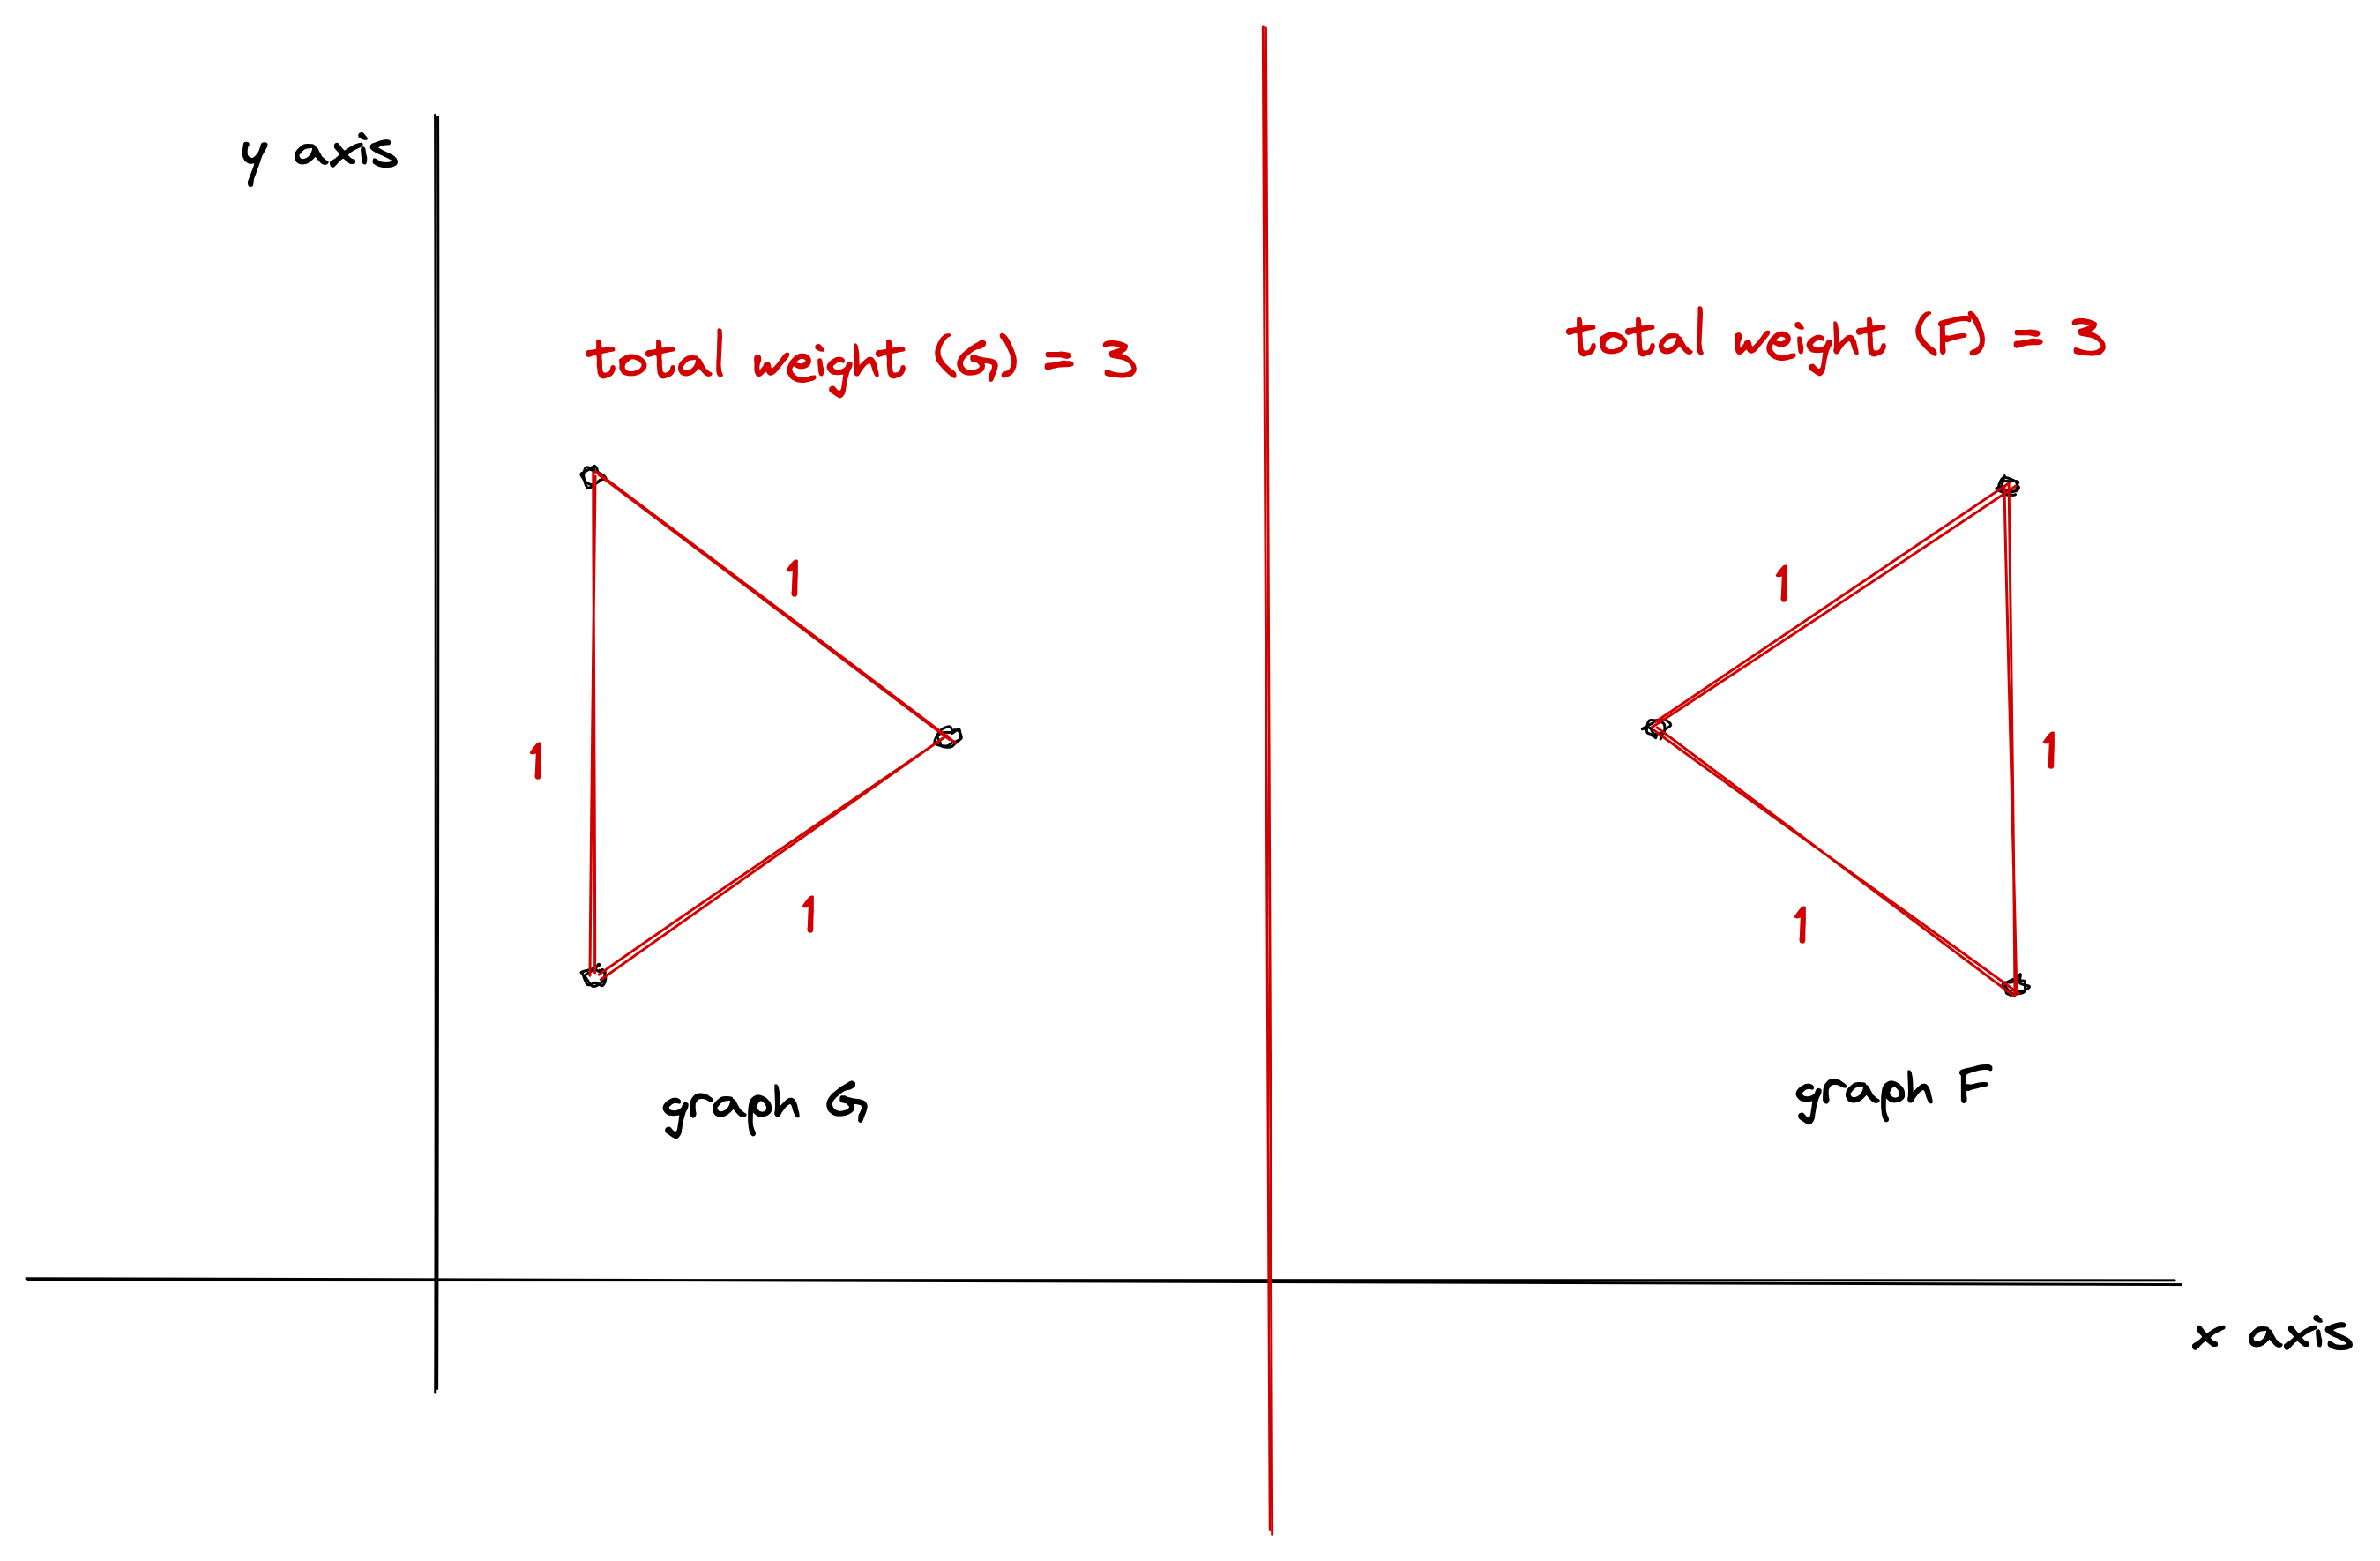
\includegraphics[scale=0.13]{non-subadditive.png}

    When considered the individual graphs, the each of the individual \textsf{NGA} output is 3.
    So $\textsf{NGA}(F) + \textsf{NGA}(G) = 6$.

    Let's consider the union of the two graphs $G \cup F$. The tour cost is $> 6$.
    Our \textsf{NGA} algorithm will choose AB, BC, DE, EJ edges first. Then it will not
    consider AC or the DJ edge because it'll violate the if condition in Algorithm~\ref{alg:1}'s line number 4.

    That's why it'll first consider the edge CD and at the end AJ to complete the tour.

    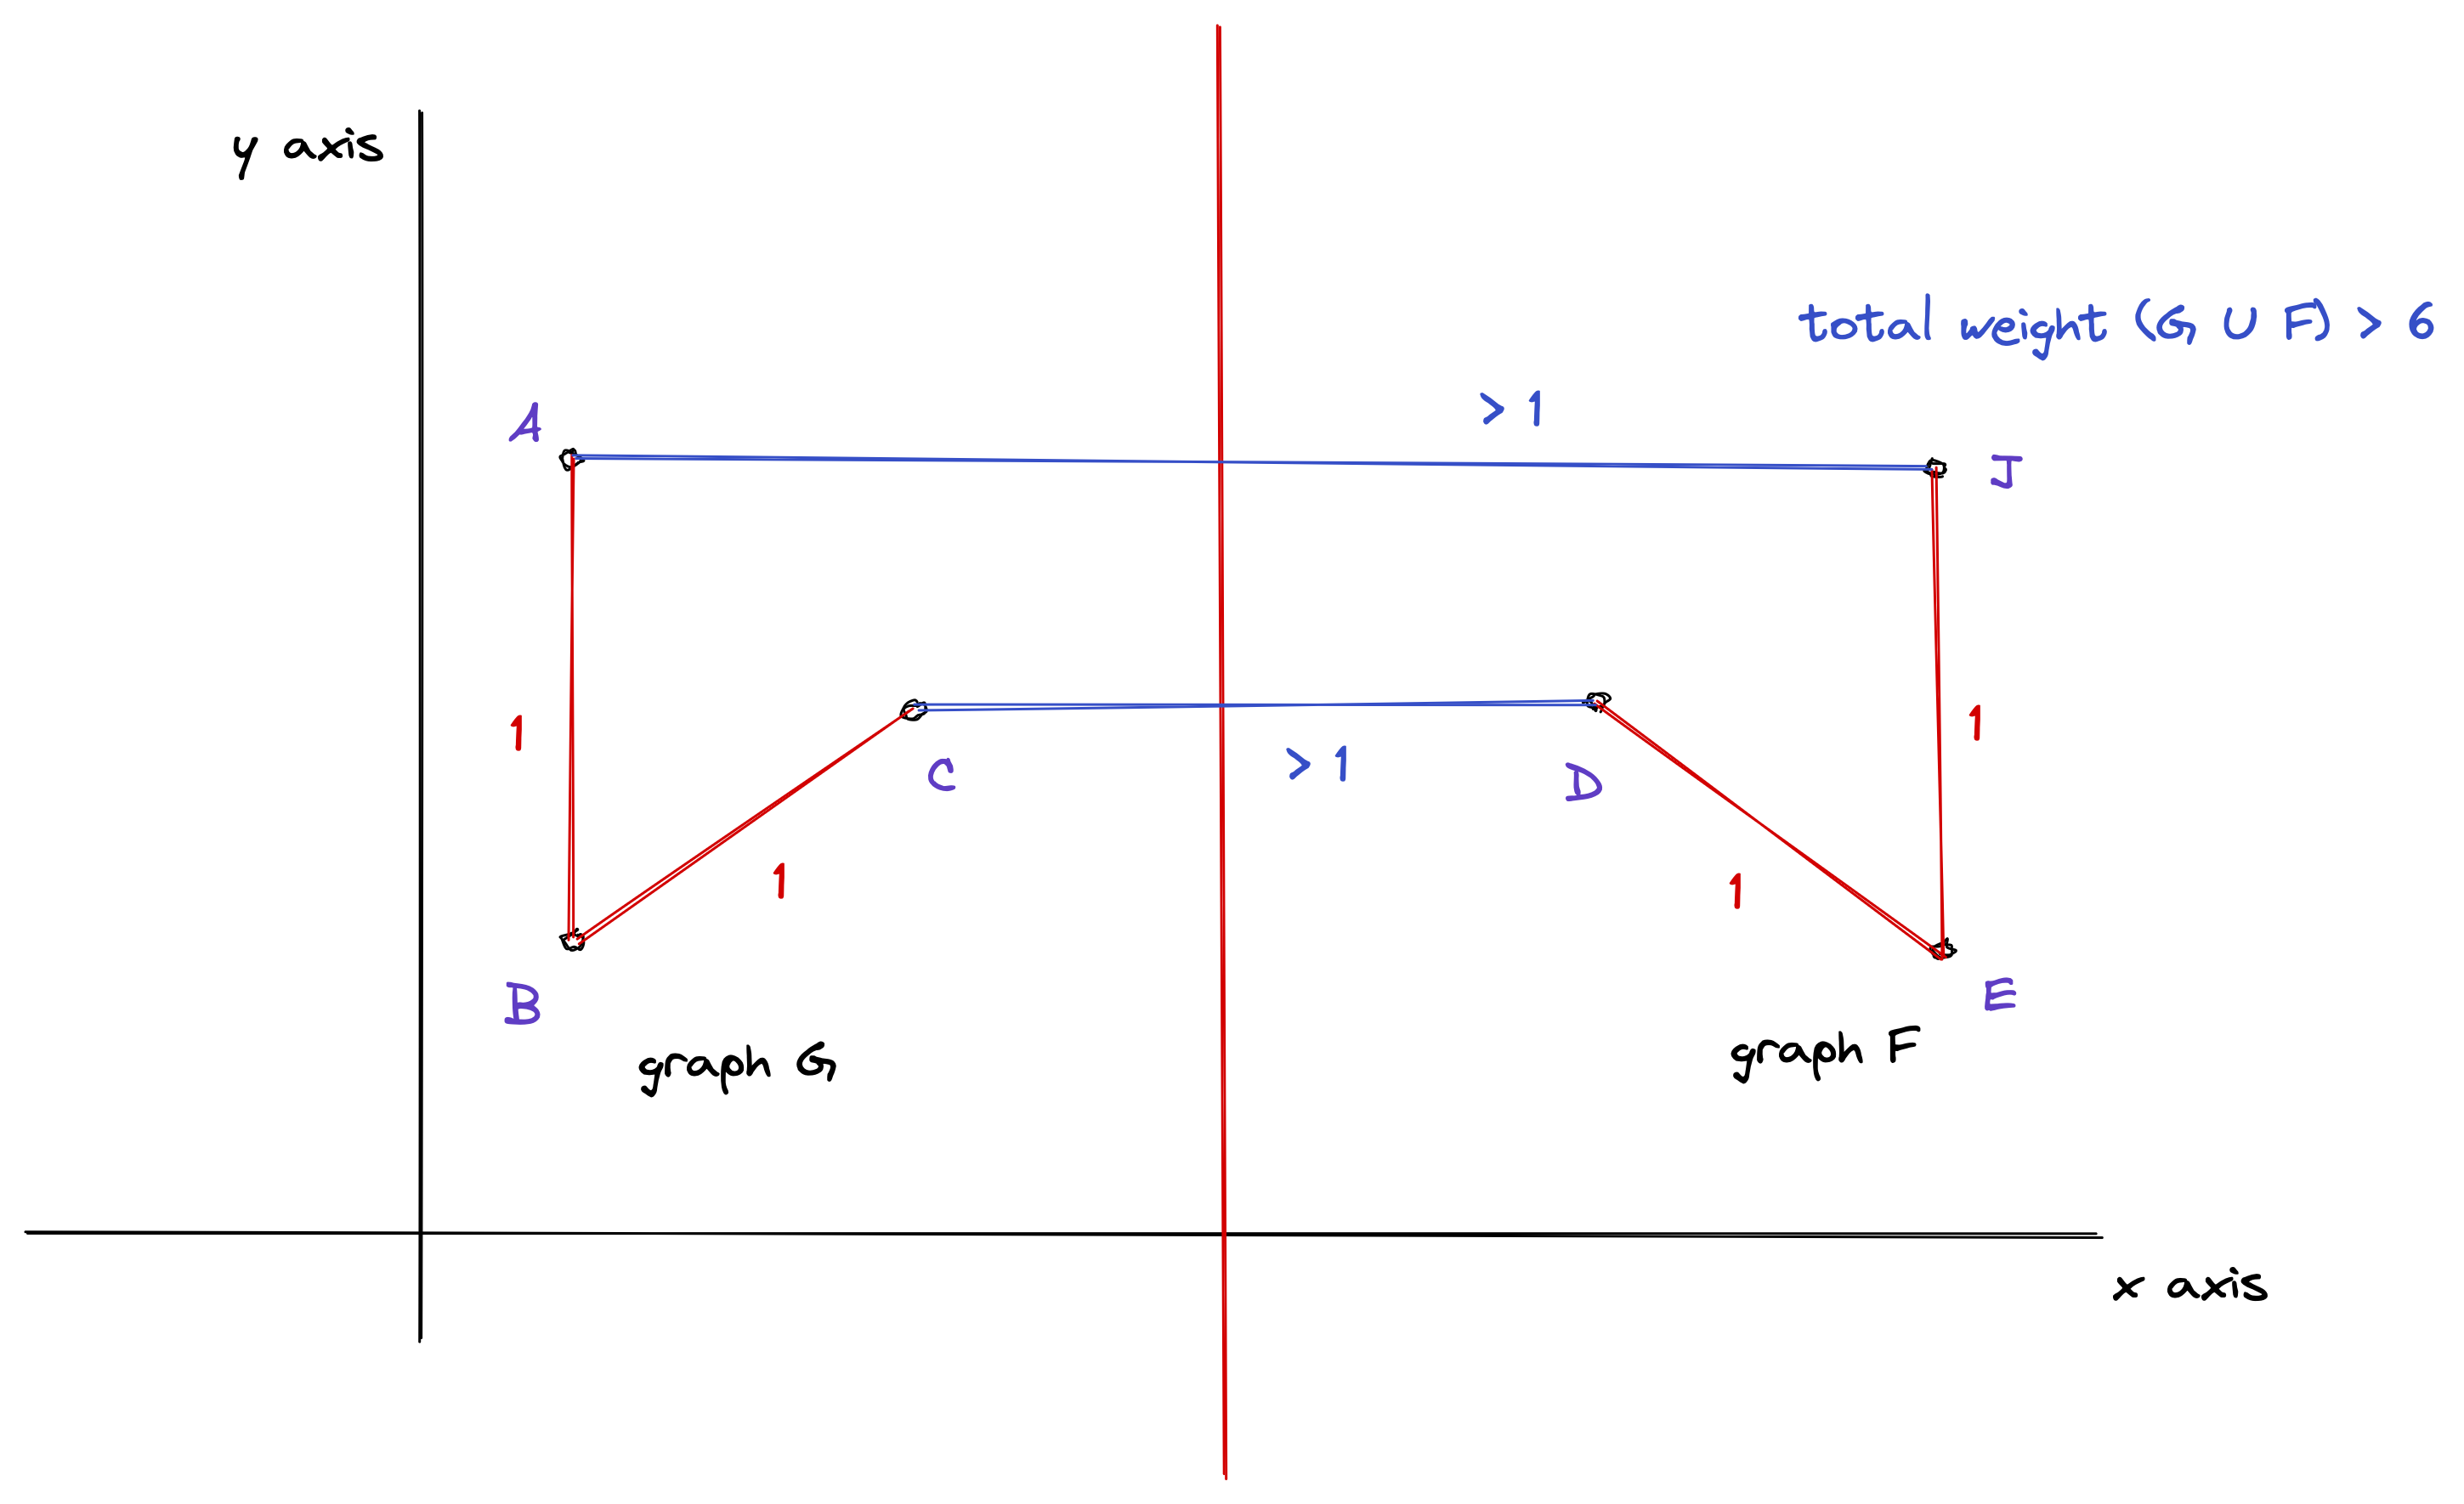
\includegraphics[scale=0.13]{non-subadditive2.png}
\end{proof}

% Example to show that simple subadditivity do not hold [small example]


\subsection{Smoothness and Monotonicity Properties}

Smoothness as defined in Yukitch's Book is given below.

\begin{define}{Smoothness}
    \textit{An euclidean functional $f$ is said to be smooth if $f(X \cup Y) - f(X)\leq c\mid Y\mid^{\frac{d-1}{d}}$
        $\forall$ $S, T \in \left[0,1 \right]^d$}.
\end{define}

If a functional is monotone then we can easily prove that the functional along
with subadditivity shows smoothness. So we explore the monotonicity of
$\textsf{NGA}$ algorithm.

An euclidean functional of representing some graph algorithm is said to be showing monotonicity if reducing points from a graph reduces the functional value.
If an euclidean functional is showing monotonicity then with subadditivity and growth bound euclidean functional shows smoothness.

\begin{define}{Monotonicity}
    \textit{If $F \subseteq G$ in some arbitrary region $\mathcal{H}$ then an monotone euclidean function
    must hold the following inequality $f(F, \mathcal{H}) \leq f(G, \mathcal{H})$}
\end{define}

\begin{lemma}
    Our \textsf{NGA} functional do not show monotone property according to the definition above. This can be proved
    by the following family of counter example below.
\end{lemma}

\begin{proof}
    We prove this by constructing a counter example.
\end{proof}

\end{document}